% COS711 Assignment 1 report. Build:  cd report && tectonic main.tex
% Figures are produced by notebook section 5 (figures/report/*.pdf).
\documentclass[10pt,a4paper]{article}
\usepackage[margin=1.8cm]{geometry}
\usepackage[T1]{fontenc}
\usepackage{lmodern}
\usepackage{microtype}
\usepackage{graphicx}
\usepackage{booktabs}
\usepackage{amsmath}
\usepackage{enumitem}
\usepackage[font=small,labelfont=bf]{caption}
\usepackage[hidelinks]{hyperref}
\usepackage[compact,small]{titlesec}
\setlength{\textfloatsep}{8pt plus 2pt minus 2pt}
\setlength{\floatsep}{6pt plus 2pt minus 2pt}
\captionsetup{skip=3pt}
\graphicspath{{../figures/report/}}
\setlist{nosep,leftmargin=*}
\setlength{\parskip}{0.3em}
\setlength{\parindent}{0pt}
\newcommand{\A}{\,\text{\AA}}

\title{\vspace{-1.5em}\textbf{Learning-Rate Warmup and Pruning Robustness\\in an MLP for Protein Structure Quality Prediction}\vspace{-0.5em}}
\author{Kyle Liebenberg \quad u22608789 \quad COS711 Assignment 1} 
\date{\vspace{-1.5em}}

\begin{document}
\maketitle

\section{Introduction}
We train multilayer perceptrons (MLPs) on the \emph{Physicochemical Properties of Protein Tertiary
Structure} dataset~[4] (UCI id 265, from the CASP experiments). Each row is a candidate 3D structure
(a \emph{decoy}) of a protein, described by nine physicochemical features (F1--F9). The target is its
RMSD, the deviation from the true structure in ångströms (\A). The task is regression: estimate how wrong a
decoy is without knowing the true structure. We first study three MLP design axes (optimiser,
architecture, activation function), and then test whether learning-rate warmup improves robustness to
magnitude pruning, and whether it does so by enabling a larger learning rate. For every experiment,
the hypotheses and decision rules were written and committed to version control \emph{before} it ran.
All numbers are reproducible from the accompanying notebook.

\section{Data preparation}
\begin{figure}[h]
  \centering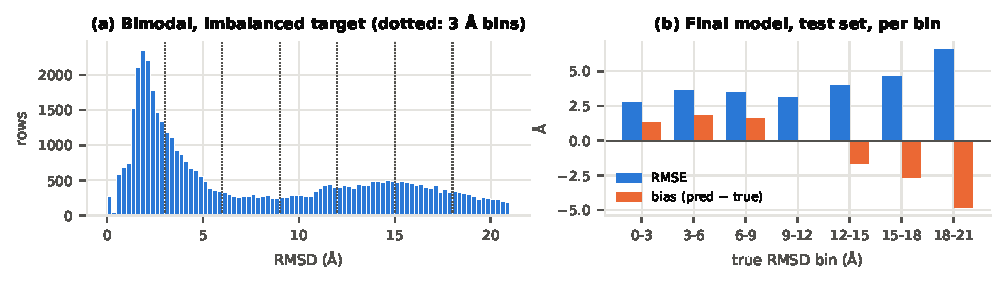
\includegraphics[width=\linewidth]{fig1_data.pdf}
  \vspace{-1.5em}
  \caption{(a) The target is bimodal: a near-native peak at 1--3\A{} and a broad hump at 11--17\A{}.
  (b) The final model's test error and bias (prediction $-$ truth) per RMSD bin.}
  \label{fig:data}
\end{figure}

\textbf{Cleaning.} 1{,}711 exact duplicate rows (3.7\%) were removed before splitting, leaving
44{,}019 rows. A duplicate on both sides of a split would leak training rows into evaluation.

\textbf{Feature relevance.} Linear correlation with RMSD is near zero for most features, yet every
feature's mutual information (MI, 0.18--0.35) is far above that of a random-noise column (0.000). F7,
for example, has $r=-0.003$ but the highest MI. The relationships are non-linear, so a correlation filter
would wrongly discard useful features, and \textbf{no feature is uninformative}. Two features are nearly
redundant. \textbf{F2 = F1\,$\times$\,F3 exactly} (non-polar exposed area = total area $\times$ non-polar
fraction), so it was dropped. F5 $\approx 138.5\times$F1 was dropped at first too, but its small deviation
(F5/F1, roughly the mean mass of the exposed residues) has MI 0.089. An MLP with F5 beat one without
it in 5/5 seeds (CV RMSE 4.10 vs 4.15\A), so F5 was restored. This gives \textbf{8 inputs}. Lesson: redundancy
depends on the model (a tree model had missed this).

\textbf{Outliers.} Six features are right-skewed (skew $>1$). On such data the IQR rule mostly flags
the natural long tail. After \texttt{log1p}, almost all flags vanish except for F7, whose maximum is
$\sim$28$\times$ its median. Those rows have ordinary RMSD values, so they were kept. Instead, every
feature is \textbf{log-transformed (if skewed) and clipped to its training 0.5th--99.5th percentile}. The
target is never clipped, because a large RMSD is a genuine bad decoy.

\textbf{Scaling.} Features are standardised (z-scores), as is the target for training. Metrics are
reported in \A. Z-scores were preferred to min-max scaling because they are zero-centred (all-positive
inputs force a neuron's weight gradients to share a sign), they match the unit-variance assumption of
Xavier/He initialisation, and they keep sigmoid/tanh out of saturation. Every transform is fitted on
training data only.

\textbf{Splitting.} An 80/20 train/test split (35{,}215 / 8{,}804 rows), \emph{stratified on 3\A{} RMSD
bins}, with a fixed seed. The test set was used only for the final results. All model comparisons use
5-fold stratified cross-validation (CV) on the training set, and 10\% of each fold's training part is held out for
early stopping, so the stopping epoch is never chosen on scored data. Limitation: there are no protein IDs, so
decoys of the same protein can appear on both sides of a split.

\textbf{Imbalance.} The 0--3\A{} bin holds 34\% of rows and the 18--21\A{} bin 7\% (Fig.~\ref{fig:data}a).
It is handled through stratified folds and test split, and through \emph{per-bin} RMSE and bias at evaluation.
Inverse-bin-frequency loss weights were tested and rejected. They cut rare-bin error by up to 0.54\A{} but
added 1.0\A{} in the common 0--3\A{} bin, and overall RMSE rose from 4.09 to 4.31\A. Nor did they remove the
under-prediction of high RMSD, which stems from the features, not the loss.

\section{Core investigation}
\textbf{Baseline.} A 2$\times$64 ReLU MLP (He initialisation, Adam with learning rate (LR) $10^{-3}$, batch 256, early stopping with patience 20)
reaches CV RMSE \textbf{4.09\A} ($R^2=0.555$). For comparison: predicting the mean gives 6.14\A, linear regression 5.19\A{}
($R^2=0.29$), and gradient-boosted trees 4.13\A. Each axis below changes one setting, with 3 seeds $\times$ 5
folds per configuration. \emph{Convergence speed} is the number of epochs until the early-stopping MSE
(on standardised RMSD, where predicting the mean scores 1.0) drops below 0.50.

\begin{figure}[t]
  \centering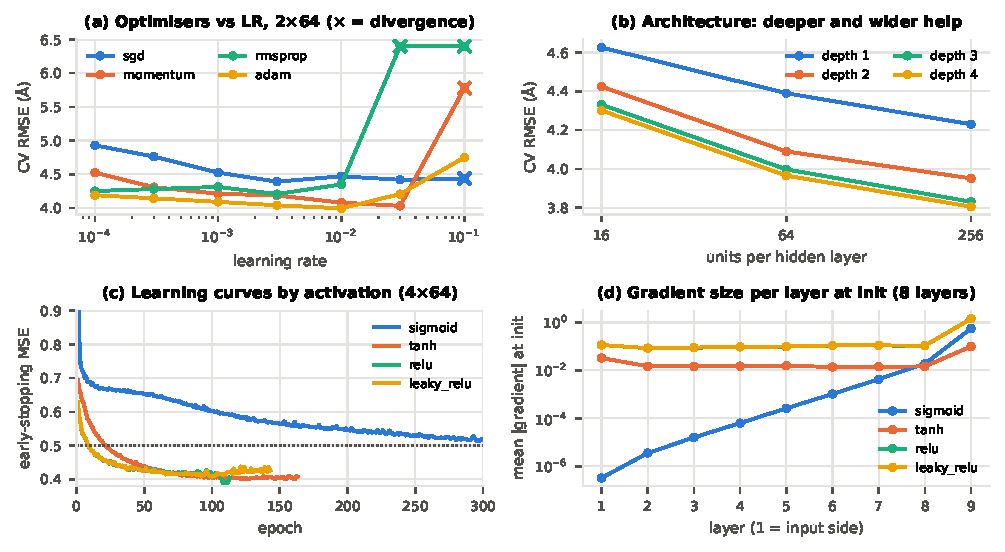
\includegraphics[width=\linewidth]{fig2_core.pdf}
  \vspace{-1.6em}
  \caption{Core investigation (CV on the training set, mean of 3 seeds). (a) Each optimiser across a shared LR grid.
  (b) RMSE by depth and width. (c) Early-stopping learning curves by activation. (d) Mean gradient
  magnitude per layer at initialisation, 8 hidden layers. ReLU and Leaky ReLU overlap.}
  \label{fig:core}
\end{figure}

\begin{table}[t]
\centering\small
\begin{tabular}{@{}p{0.47\linewidth}p{0.48\linewidth}@{}}
\toprule
Hypothesis (stated before running) & Verdict and evidence \\
\midrule
A1: Adam/RMSprop converge fastest, SGD slowest & \textbf{Partly.} Epochs to 0.50: Adam 9.7, momentum 12.5, RMSprop 29.5, SGD 293 \\
A2: at best LRs, all optimisers within 0.05\A & \textbf{Contradicted.} Adam 3.99, momentum 4.03, RMSprop 4.21, SGD 4.39\A \\
A3: adaptive methods tolerate more LRs; momentum fails before SGD & \textbf{Mixed.} Adam most tolerant, RMSprop \emph{least}; momentum fails at 0.1, SGD does not \\
B1: width 16$\to$64 helps, 64$\to$256 $<$0.05\A & \textbf{Partly.} $-$0.33 then $-$0.14\A \\
B2: 2 layers beat 1; more adds $<$0.05\A & \textbf{Half.} 1$\to$2: $-$0.30\A; 2$\to$4: $-$0.12\A \\
B3: big nets overfit sooner; early stopping protects them & \textbf{Supported.} Best epoch 310$\to$54; best net is 4$\times$256 (3.81\A) \\
C1: speed ReLU $>$ tanh $>$ sigmoid & \textbf{Supported.} 8.6 / 21 / 340 epochs (4$\times$64) \\
C2: sigmoid gradients vanish with depth (softened by Adam) & \textbf{Supported.} $\approx$4$\times$ shrink per layer; affects speed more than final RMSE \\
C3: tanh $\approx$ ReLU $\approx$ Leaky ReLU & \textbf{Partly.} Leaky = ReLU ($<$0.5\% dead units); tanh beat ReLU at depth 4 (3.90 vs 3.97\A) \\
\bottomrule
\end{tabular}
\caption{Core-investigation hypotheses and verdicts. A difference counted only if it exceeded seed/fold noise ($\sim$0.015/0.04\A) in all seeds.}
\label{tab:core}
\end{table}

\textbf{Optimisers} (Fig.~\ref{fig:core}a). Momentum gave a $\sim$20$\times$ speed-up over plain SGD and
beat RMSprop, so much of Adam's speed seems to come from the momentum it contains. Final quality was
\emph{not} equal (A2 contradicted). Under a fixed budget and early stopping, plain SGD never reached the good
region: at small LRs its best epoch was the 500-epoch limit. RMSprop was the most fragile optimiser at
high LRs (it diverged at $\geq 3\cdot10^{-2}$). We measured why: PyTorch's RMSprop has no bias correction, so its
first update is 10$\times$ the LR, against 1$\times$ for Adam. Oversized early steps are exactly the problem warmup
addresses. Large LRs also killed ReLU units (Adam: 0.3\% dead at $10^{-3}$, 48\% at $10^{-1}$).

\textbf{Architecture} (Fig.~\ref{fig:core}b). Every increase in width or depth lowered RMSE, consistently across
seeds. Bigger nets overfit sooner (larger train--validation gap), but early stopping halted them first, so
the largest net was best. Depth was more parameter-efficient: 4$\times$64 (13k weights) matched 2$\times$256 (68k).
Hypotheses B1/B2 under-estimated capacity because they assumed a ``feature ceiling'' suggested by MLP and
trees both stopping at $R^2\approx0.55$. That ceiling was really the baseline's limited capacity.

\textbf{Activations} (Fig.~\ref{fig:core}c,d). Sigmoid's gradients shrink by $\approx$4$\times$ per layer going
backwards, matching its maximum derivative of 0.25, and reach $\sim$$10^{-6}$ of the output layer's after 8 layers.
tanh and ReLU keep gradients flat. With Adam, which rescales each weight's step by its own gradient scale,
this shows up as slow training (340 vs 8.6 epochs) rather than failure.

\textbf{Final test evaluation.} The best CV-validated configuration (4$\times$256, ReLU, Adam $10^{-3}$) reaches
\textbf{test RMSE $3.78\pm0.03$\A, $R^2=0.621$} (5 seeds), in close agreement with its CV score (3.81\A), so model selection
did not overfit the validation folds. Per bin (Fig.~\ref{fig:data}b), errors grow towards the rare high-RMSD bins,
with regression to the mean: over-prediction of +1.3\A{} for 0--3\A{} and under-prediction of $-$4.8\A{} for 18--21\A.

\section{Research investigation: warmup and pruning robustness}
\textbf{Design.} The network is 4$\times$256 ReLU, trained with SGD with momentum 0.9 (batch 256) for a fixed 100 epochs with cosine decay. Warmup
adds a linear ramp over the first 5 epochs. Choices are made on a 10\% validation split, and all pruning results are reported on the
test set, over 5 seeds. \textbf{Step 1:} train with and without warmup over an LR grid
(0.005--0.2). \textbf{Step 2:} pre-registered rules choose \textbf{A} (no warmup, at its best LR $\eta_0$),
\textbf{B} (warmup, at the largest LR $>\eta_0$ whose validation RMSE is within 0.05\A{} of A's: \emph{comparable
unpruned accuracy}) and the control \textbf{C} (warmup at $\eta_0$). \textbf{Step 3:} one-shot \emph{global
magnitude pruning} of all weight matrices at 0--98\% sparsity, followed by identical fine-tuning (LR 0.001, 10 epochs,
pruned weights held at 0 by masks). Robustness is $\Delta(s)$ = test RMSE after fine-tuning minus unpruned test RMSE.
\textbf{Hypotheses:} \textbf{H1}: warmup raises the maximum stable LR. \textbf{H2}: B has a smaller $\Delta$ than A at
sparsities $\geq$70\%. \textbf{H3}: the benefit comes from the larger LR, so B beats C while C $\approx$ A.

\begin{figure}[t]
  \centering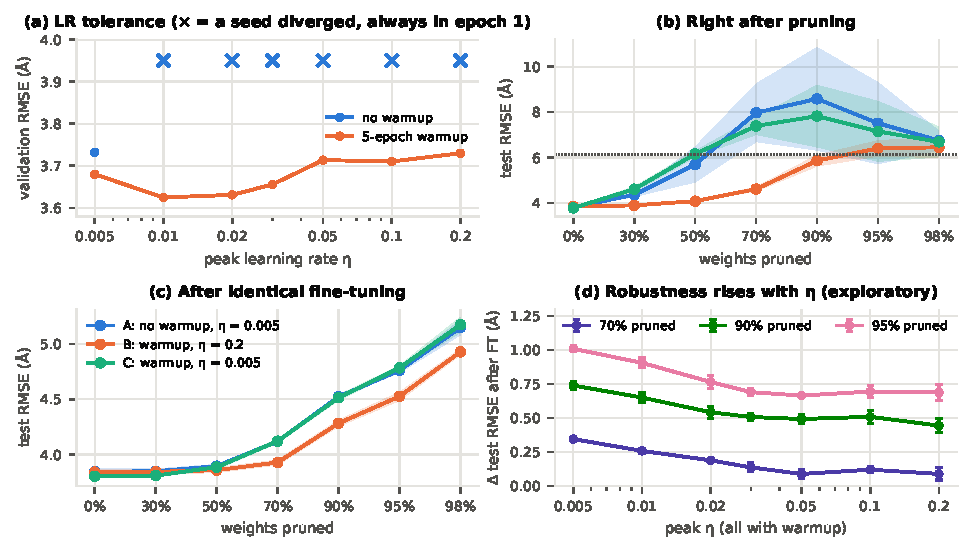
\includegraphics[width=\linewidth]{fig3_warmup_pruning.pdf}
  \vspace{-1.6em}
  \caption{Warmup and pruning (mean $\pm$ std over 5 seeds; (b)--(d) on the test set). (a) Validation RMSE vs peak LR; $\times$ = at least one seed diverged.
  (b, c) Accuracy vs sparsity for conditions A, B, C, before and after identical fine-tuning (dotted: predicting the mean).
  (d) Exploratory: $\Delta$ vs peak LR among warmup-trained networks.}
  \label{fig:warmup}
\end{figure}

\begin{table}[t]
\centering\small
\begin{tabular}{@{}lcccccc@{}}
\toprule
& Unpruned test RMSE & $\Delta$ 70\% & $\Delta$ 90\% & $\Delta$ 95\% & $\Delta$ 98\% & Dead units \\
\midrule
A: no warmup, LR 0.005 & 3.81 & 0.31 & 0.71 & 0.95 & 1.34 & 3.6\% \\
B: warmup, LR 0.2      & 3.84 & \textbf{0.09} & \textbf{0.44} & \textbf{0.69} & \textbf{1.09} & 0.2\% \\
C: warmup, LR 0.005    & 3.78 & 0.35 & 0.74 & 1.01 & 1.40 & 0.0\% \\
\bottomrule
\end{tabular}
\caption{Error added by pruning after fine-tuning ($\Delta$, \A; mean of 5 seeds). B vs A: $-$0.22 to $-$0.27\A{} and
B vs C: $-$0.26 to $-$0.32\A, smaller in 5/5 seeds at every sparsity. C vs A: $+$0.03 to $+$0.06\A{}, with C better in only 0--2/5 seeds.}
\label{tab:prune}
\end{table}

\textbf{H1: supported.} Without warmup, the largest stable LR was 0.005. At 0.01, 2/3 seeds diverged, and at
$\geq$0.02 all did, \emph{every time within the first epoch}. With warmup all runs trained, up to 0.2
(Fig.~\ref{fig:warmup}a), a $\geq$20$\times$ increase. This is consistent with Kalra and Barkeshli~[3]: small early steps move the
network to a better-conditioned region, where large steps are safe. The rules selected $\eta_0=0.005$ and, for B,
LR 0.2 (validation RMSE 3.73 vs 3.74\A). Warmup at 0.01--0.03 was $\sim$0.1\A{} \emph{better} than A and therefore not
``comparable''.

\textbf{H2 and H3: supported} (Table~\ref{tab:prune}, Fig.~\ref{fig:warmup}b,c). At matched unpruned accuracy
(B's test RMSE was even slightly worse), B lost 0.22--0.27\A{} less than A, in 5/5 seeds at every sparsity $\geq$70\%.
Right after pruning the gap is dramatic: at 70\% sparsity B's RMSE is 4.6\A, while A and C jump to 8.0 and 7.4\A,
worse than predicting the mean. The control is decisive. Warmup at the small LR (C) brought \emph{no} benefit,
so warmup helps only through the larger LR it enables. Alternative explanations were checked:
B had the \emph{fewest} dead units, so its pruning was not ``free'' sparsity. The fine-tuning LR was
relatively larger for A and C, which should favour their recovery~[2]. And measuring $\Delta$ against the fine-tuned
dense network gives the same ranking.

\textbf{Extensions.} \emph{(E3, exploratory, Fig.~\ref{fig:warmup}d)} Among warmup-trained networks, robustness
rises steadily with the peak LR: $\Delta_{70\%}$ falls from 0.35 to 0.09\A{} (Spearman $\rho=-0.88$ over 35 runs), even
though LR 0.01 gives the best \emph{unpruned} model. Robustness tracks the LR, not the starting accuracy.
\emph{(E1)} Retraining with each network's own schedule (LR rewinding~[2]) instead of fine-tuning improved recovery for all
conditions, but \emph{widened} the A--B gap (B lost only 0.03\A{} at 90\% vs 0.58\A{} for A), contrary to our prediction.
The large LR helps twice: it gives more robust weights and more effective retraining. \emph{(E2)} One epoch of warmup already
made LR 0.2 trainable. A 15-epoch warmup was \emph{less} robust than a 5-epoch one (4--5/5 seeds), plausibly because it leaves fewer
epochs at the large LR. A post-hoc look at the weights suggests one reason large-LR networks prune well: B
concentrates more of its weight mass in its largest weights (top 10\% hold 60.6\% of $\sum w^2$ vs 56.5\% for A).

\textbf{Interpretation and limitations.} We observed the effect reported by Frankle and Carbin~[1], and the evidence
supports the proposed mechanism on both links. Warmup raises the tolerable LR (H1), and the larger LR, not
warmup itself, produces the robustness (H3, E3). Warmup's effect on pruning robustness is therefore
\emph{indirect}. Limitations: a single tabular dataset with an MLP (the original studies used CNNs on images),
one-shot rather than iterative pruning, a single fit/validation split, and B's LR lying at the edge of the grid. Large-LR
training without warmup cannot be tested, because it diverges. Finally, the reason large-LR networks are robust (weight
concentration or flatter minima) was explored only post hoc.

\section{Conclusion}
Careful data preparation (log transform, clipping, stratification, per-bin evaluation, and checking feature
decisions with the model itself) gave a 4$\times$256 MLP with test RMSE 3.78\A{} ($R^2=0.62$). Capacity, optimiser
choice and LR mattered more than our initial hypotheses expected, and sigmoid's vanishing gradients appeared exactly as
theory predicts. In the research investigation, warmup raised the tolerable LR at least 20-fold. At matched accuracy,
the warmup-trained network was clearly more robust to magnitude pruning, but only because of the larger LR that
warmup unlocks.

\begin{thebibliography}{4}\footnotesize\setlength{\itemsep}{0pt}
\bibitem{lth} J.~Frankle and M.~Carbin, ``The lottery ticket hypothesis: Finding sparse, trainable neural networks,'' in \emph{Proc.\ ICLR}, 2019.
\bibitem{renda} A.~Renda, J.~Frankle, and M.~Carbin, ``Comparing rewinding and fine-tuning in neural network pruning,'' in \emph{Proc.\ ICLR}, 2020.
\bibitem{kalra} D.~S.~Kalra and M.~Barkeshli, ``Why warmup the learning rate? Underlying mechanisms and improvements,'' in \emph{Advances in NeurIPS}, 2024.
\bibitem{uci} ``Physicochemical Properties of Protein Tertiary Structure,'' UCI Machine Learning Repository, dataset 265. \url{https://archive.ics.uci.edu/dataset/265}.
\end{thebibliography}

\end{document}
